%!TEX root=../main.tex

\section*{Аннотация}

\vspace{-0.5cm}
Алгоритмы планирования задач на вычислительных кластерах являются предметом активных исследований. Проведение таких исследований на настоящем кластере долго и дорого, поэтому для сравнения различных гипотез используются симуляторы. Качество получаемых результатов во многом зависит от точности используемой модели. Большинство современных симуляторов используют простые компьютерные модели, которых не всегда достаточно. Эта работа сосредоточена на разработке симулятора вычислительного кластера на базе фреймворка DSLab, который позволит очень точно и гибко моделировать сценарии вычислительной нагрузки с использованием примитивов асинхронного программирования. DSlab предоставляет массу возможностей как для написания новых алгоритмов, так и для использования готовых модулей различных компонент распределенной системы. Таким образом, новый симулятор получит основные преимущества DSlab, которые сделают его еще более привлекательным для исследователей сложных алгоритмов.

\vspace{-0.5cm}
\section*{Ключевые слова}

Распределенные системы, вычислительный кластер, алгоритмы планирования, симуляция, DSLab
\vspace{-0.5cm}
\section*{Annotation}
\vspace{-0.5cm}
Algorithms for scheduling tasks on compute clusters are the subject of active research. It is quite expensive to conduct such studies using real cluster, so simulators are used to compare different hypotheses. The quality of the results obtained largely depends on the accuracy of the model used. Most modern simulators use simple compute models, which are not always enough. Our work is focused on developing a simulator of a compute cluster based on the DSLab framework, which will allow very accurate and flexible modeling of computational load scenarios using asynchronous programming primitives. DSLab provides a lot of opportunities both for writing new algorithms and using ready-made modules of various distributed system components. Thus, the new simulator will receive the basic advantages of DSLab, which will make it even more attractive for researchers of complex algorithms.


\vspace{-0.5cm}
\section*{Keywords}
Distributed systems, compute cluster, scheduling algorithms, simulations, DSLab 

\newpage 

\section{Введение}

Вычислительные кластеры, состоящие из набора серверов с различными ресурсами (процессор, память, диск), широко применяются для проведения сложных расчетов и обработки больших объемов данных в науке и бизнесе. На большом промышленном кластере одновременно могут выполняться тысячи заданий (batch jobs) различных пользователей, а часть заданий может находиться в очереди в ожидании выделения ресурсов. Запуском заданий и распределением ресурсов между ними управляет менеджер кластера или планировщик. В основе работы менеджера кластера лежат алгоритмы планирования задания (job scheduling), основной целью которых является максимально эффективное использование ресурсов кластера. Данные алгоритмы являются предметом активных исследований. Проводить такие исследования на реальном кластере долго и дорого, поэтому необходима компьютерная модель (симулятор), позволяющая быстро проверить гипотезу или провести сравнительное тестирование разных алгоритмов на некоторой истории нагрузки кластера. Подобный симулятор также может использоваться в учебном процессе для знакомства студентов с такими системами и возникающими в них задачами.

\subsection{Актуальность и значимость}

% Фреймворк DSLab предоставляет большие возможности для написания различных симуляций.

\subsection{Цели и задачи ВКР}

Целью ВКР является разработка симулятора вычислительного кластера на базе фреймворка DSLab. 

Для достижения этой цели были поставлены следующие задачи: 
\begin{enumerate}
\item  Изучить литературу по теме и существующие симуляторы, подготовить обзор с анализом их преимуществ и недостатков.
\item Поэтапно реализовать компоненты симулятора, покрыть их тестами и снабдить комментариями.
\item Подготовить и провести эксперименты, демонстрирующие работоспособность симулятора и достижение всех требований.
\item Подготовить документацию пользователя.
\end{enumerate}

\subsection{Основные результаты работы}

\subsection{Структура работы}

\section{Обзор литературы}

\subsection{Вычислительная модель}

Для моделирования работы кластера и алгоритмов планирования требуется модель рабочей нагрузки. Standard Workload Format(SWF)\cite{standard-workload-format} широко используется в литературе и поддерживается многими симуляторами. Однако, SWF предоставляет довольно мало информации о рабочей нагрузке. Ключевая информация о единице рабочей нагрузки <<Job>> включает время прибытия, время выполнения, приоритет и потребность в ресурсах. Единственное предположение, которое мы можем сделать относительно рабочей нагрузки заключается в том, что <<Job>> потребляет все заданные ресурсы во время выполнения. Наиболее популярные трейсы рабочей нагрузки представлены в аналогичном формате (например, Google trace\cite{google-clusterdata}).

Однако, существует и более сложный подход к моделированию задач на кластере, при котором время выполнения задачи рассчитывается на основе структуры рабочей нагрузки и доступных ресурсов. Основное преимущество этого подхода заключается в том, что больше деталей задачи могут быть учтены и использованы при планировании. Кроме того, появляется возможность с большей точностью рассчитать загрузку кластера и поведение его компонент. Основной недостаток -- для такого моделирования довольно сложно найти данные из открытых источников, поскольку информация о детальной структуре задач обычно конфиденциальна и не публикуется.

\subsection{Аналоги}

Существующие симуляторы относятся к одной из двух категорий: симуляторы, созданные с нуля, и основанные на готовой платформе. Другой способ группировки симуляторов -- по типу рабочей нагрузки, которую они поддерживают: симуляторы, которые работают с SWF или аналогичными форматами, и поддерживающие сложное описание рабочей нагрузки.

\subsubsection{AccaSim}

Характерным примером такого симулятора <<с нуля>> является AccaSim\cite{accasim-article}. Он основан на дискретно-событийном моделировании и содержит предопределенные алгоритмы планирования. Он довольно прост в использовании, но не поддерживает сложные конфигурации. В отличие от AccaSim, наш симулятор сможет моделировать произвольные сценарии рабочей нагрузки, которые будут определены пользователями. Кроме того, наш симулятор является модульным, поскольку основан на DSLab. Пользователи смогут подключать модули, написанные другими исследователями в рамках платформы DSLab, и использовать их в своих экспериментах. Например, DSLab предоставляет модели сети, которые могут точно симулировать различные топологии.

\subsubsection{BatSim}

Симулятор Batsim основан на SimGrid\cite{simgrid-article} и позволяет разработчикам интегрировать алгоритмы на нескольких языках на основе inter-process communication. Подробное сравнение SimGrid и DSLab можно найти в документации по DSLab\cite{dslab-analog-cmp}. Ключевое ограничение BatSim -- из возможных ресурсов кластера он поддерживает моделирование только <<вычисления>>, <<передачу данных>> и <<операции с распределенной файловой системой>>. Batsim предоставляет интерфейс для настройки пользовательских типов рабочей нагрузки, но они ограничены несколькими заданными паттернами и возможными последовательными комбинациями из них (см. рис. \ref{fig:batsim-profile}). 

\begin{figure}[h]
    \footnotesize  
\begin{jsoncode}
"jobs": [
  {"id":"simple", "subtime":1, "res": 4, "profile": "simple"},
],
"profiles": {
  /* workload profile definition */
  "simple": {
    "type": "parallel",
    "cpu": [5e6,  0,  0,  0],
    "com": [5e6,  0,  0,  0,
            5e6,5e6,  0,  0,
            5e6,5e6,  0,  0,
            5e6,5e6,5e6,  0]
  },
}
\end{jsoncode}
\caption{Пример описания нагрузки в BatSim}
\label{fig:batsim-profile}
\end{figure}

Так же из рис. \ref{fig:batsim-profile} можно увидеть, что потребность в ресурсах задачи выражается в количестве выделенных <<ресурсов>> (одно число -- количество серверов), и задача размещается на них целиком. Таким образом, существенно ограничивается планирование задач с разным профилем требований к ресурсам (задача упаковки). Стоит отметить, что каждый сервер имеет свою вычислительную мощность, а так же каким-то образом размещен в топологии сети, поэтому проблема размещения задач оптимальным образом на кластере не сводится к тривиальной. Необходимость учитывать топологию сети в такой модели -- сложная проблема планирования. Однако, проблема упаковки задач на несколько ресурсов в такой модели не рассматривается.

Наш симулятор расширит подход BatSim для определения произвольной рабочей нагрузки, но при этом предоставит больше возможностей для управления ресурсами (процессор, память, диск), а так же предоставит еще больше возможностей для описания сценария нагрузки с использованием примитивов асинхронного программирования.

\subsubsection{IRMaSim}

Дальнейшим развитием BatSim стал симулятор IRMaSim\cite{irmasim-article}. В нем отмечаются недостатки BatSim в точности моделирования вычислений и предоставляются намного более точные модели процессоров и добавляются различные модели оперативной памяти. В этом симуляторе возможно точно указать тим оперативной памяти и ее скорость, и все это будет учитываться в симуляции. Так же этот симулятор поддерживает сценарии работы с задачами глубинного обучения (Deep Reinforcement Learning). Однако, ключевое ограничение остается то же -- потребность задач в ресурсах указывается одним числом -- количеством <<ресурсов>> (серверов). По аналогии с BatSim, этот симулятор фокусируется на потреблении энегрии в процессе работы кластера и позволяет разрабатывать алгоритмы планирования, оптимизирующие энергопотребление. 

\subsubsection{Elastisim}

Симулятор Elastisim\cite{elastisim-article} также основан на SimGrid и ориентирован на гибкие рабочие нагрузки (malleable workloads). Это позволяет моделировать динамические изменения количества ресурсов, выделяемых на исполнение задач. Одна из важных особенностей Elastisim -- высокая точность моделирования задач глубокого обучения, для которых он и предназначен. Кроме этого, в Elastisim поддерживатеся моделирование передачи данных (I/O) по сети. Авторы обращают особое внимание на то, что операции I/O могут стать узким местом, поскольку объем передаваемых данных постоянно увеличивается. Выполнение каждой задачи состоит из нескольких этапов и может быть настроено с помощью файла JSON путем объединения предварительно определенного набора операций: CPU, GPU, операций I/O и дисковых операций. Это самый продвинутый симулятор из всех рассмотренных источников. Мы будем стремиться предоставить еще больше возможностей для подробного описания выполняемых задач, однако наш симулятор будет поддерживать более распространенную модель вычислений, при которой каждой задаче выделяется фиксированная аллокация ресурсов на время выполнения.

\subsection{Выводы}

Рассмотренные симуляторы решают разные задачи симуляции: симуляция упаковки задач на кластер в условиях нескольких ресурсов (AccaSim), и точная симуляция вычислительного процесса (BatSim, IRMaSim, Elastisim). При этом ни в одном симуляторе эти задачи не пересекаются. Наш симулятор разработан в более общей модели, что позволяет поддержать задачу упаковки и точное моделирование вычислений одновременно. Более того, одной из тем исследований планирования задач на кластерах является честность (в условиях, когда кластер делится между несколькими пользователями). Задача честности не рассматривалась в приведенных симуляторах, однако наш симулятор поддерживает и эту возможность.



\section{Фреймворк DSLab}


В качестве платформы для реализации симулятора выбран \texttt{DSLab} -- модульный фреймворк для моделирования и тестирования распределенных систем. Модули можно разделить на 3 группы: базовые, универсальные и специализированные (см рисунок \ref{fig:dslab_arc}). За основу взят подход дискретно-событийного моделирования, при котором компоненты симуляции обмениваются событиями через базовый низкоуровневый модуль \texttt{dslab-core}. Соответственно, пользовательская логика каждого компонента состоит из обработки входящих событий от других компонент и отправки новых. Универсальные модули могут использовать исследователями соответствующих предметных областей, например, новый симулятор использует готовые модули вычислений, сети и диска (подробнее об этом в главе \ref{cluster-model}). 

\begin{figure}[H]
    \centering
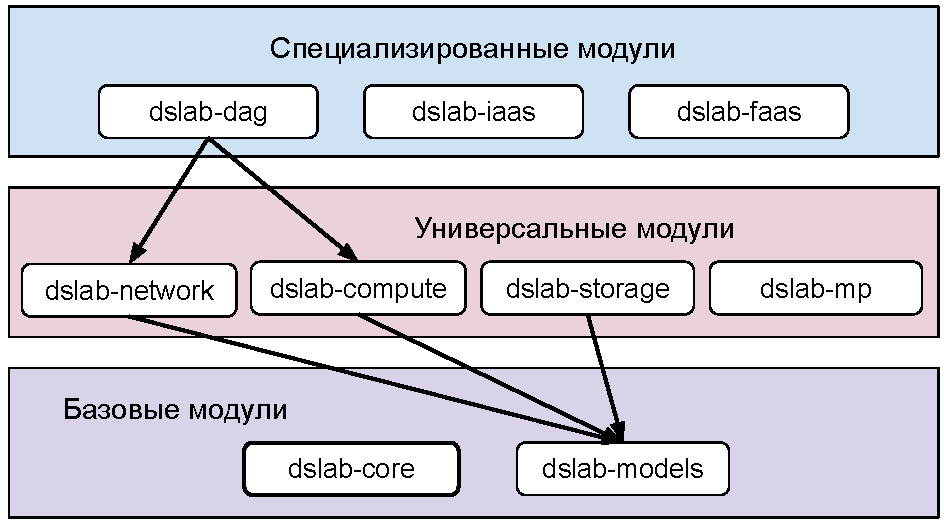
\includegraphics[width=0.7\linewidth]{images/dslab_arc}
\caption{Архитектура \texttt{DSLab}}
\label{fig:dslab_arc}
\end{figure}

Описание архитектуры основано на официальной документации \cite{dslab-architecture}. Реализация всех модулей опубликована в GitHub-репозитории\cite{dslab-repo}.

\subsection{Асинхронное управление событиями}

В предыдущей работе была добавлена возможность управлять событиями \texttt{DSLab} асинхронно\cite{async-dslab}, что существенно расширило возможности написания компонент и сделало возможным ключевую особенность нового симулятора -- описание профиля нагрузки задач через асинхронные примитивы языка \texttt{Rust} (подробнее об этом в главе \ref{compute-model}). Ключевая особенность такого расширения -- возможность спрятать от пользователя явную работу с событиями, предоставив ему высокоуровневые асинхронные функции, в реализации которых зашито асинхронное ожидание внутренних событий. Например, при работе с записью на диск можно предоставить пользователю следующую асинхронную функцию: 
\begin{figure}[h]
    \footnotesize
    \begin{rustcode}
pub async fn write_data(&self, size: u64) -> Result<(), String> {
  let req_id = self.disk.write(size, /*requester=*/self.ctx.id());

  select! {
    _ = self.ctx.recv_event_by_key::<DataWriteCompleted>(req_id).fuse() => {
        Result::Ok(())
    }
    failed = self.ctx.recv_event_by_key::<DataWriteFailed>(req_id).fuse() => {
        Result::Err(failed.data.error)
    }
  }
}
    \end{rustcode}
    \caption{Пример асинхронной функции записи данных на диск.}
\end{figure}

В этом примере используется детализированное ожидание события по ключу. Исполнение симуляции прерывается до того момента, пока компонент (в данном случае -- вычислительный сервер, на котором запущена задача) не получит событие от собственного диска о том, что запись завершилась (либо успешно, либо с ошибкой -- для альтернативного ожидания используется макрос \texttt{select!} из библиотеки \texttt{futures}\cite{rust-futures}), после этого ядро симуляции продолжит исполнение и результат вернется пользователю.  

Таким образом, пользователю не нужно будет самостоятельно следить за событиями компонент и можно будет разделить инструкции выполнения задач от конкретных компонент, предоставив лишь <<сценарий работы>> в виде асинхронных функций. 

Точно таким же образом реализованы и другие примитивы: вычисления и  работа с сетью. 


\section{Реализация симулятора}


\subsection{Архитектура симулятора}

По аналогии с самим фреймворком DSLab симулятор модульный, его архитектура представлена на рисунке \ref{fig:arch}.

\begin{figure}[h!]
    \centering 
    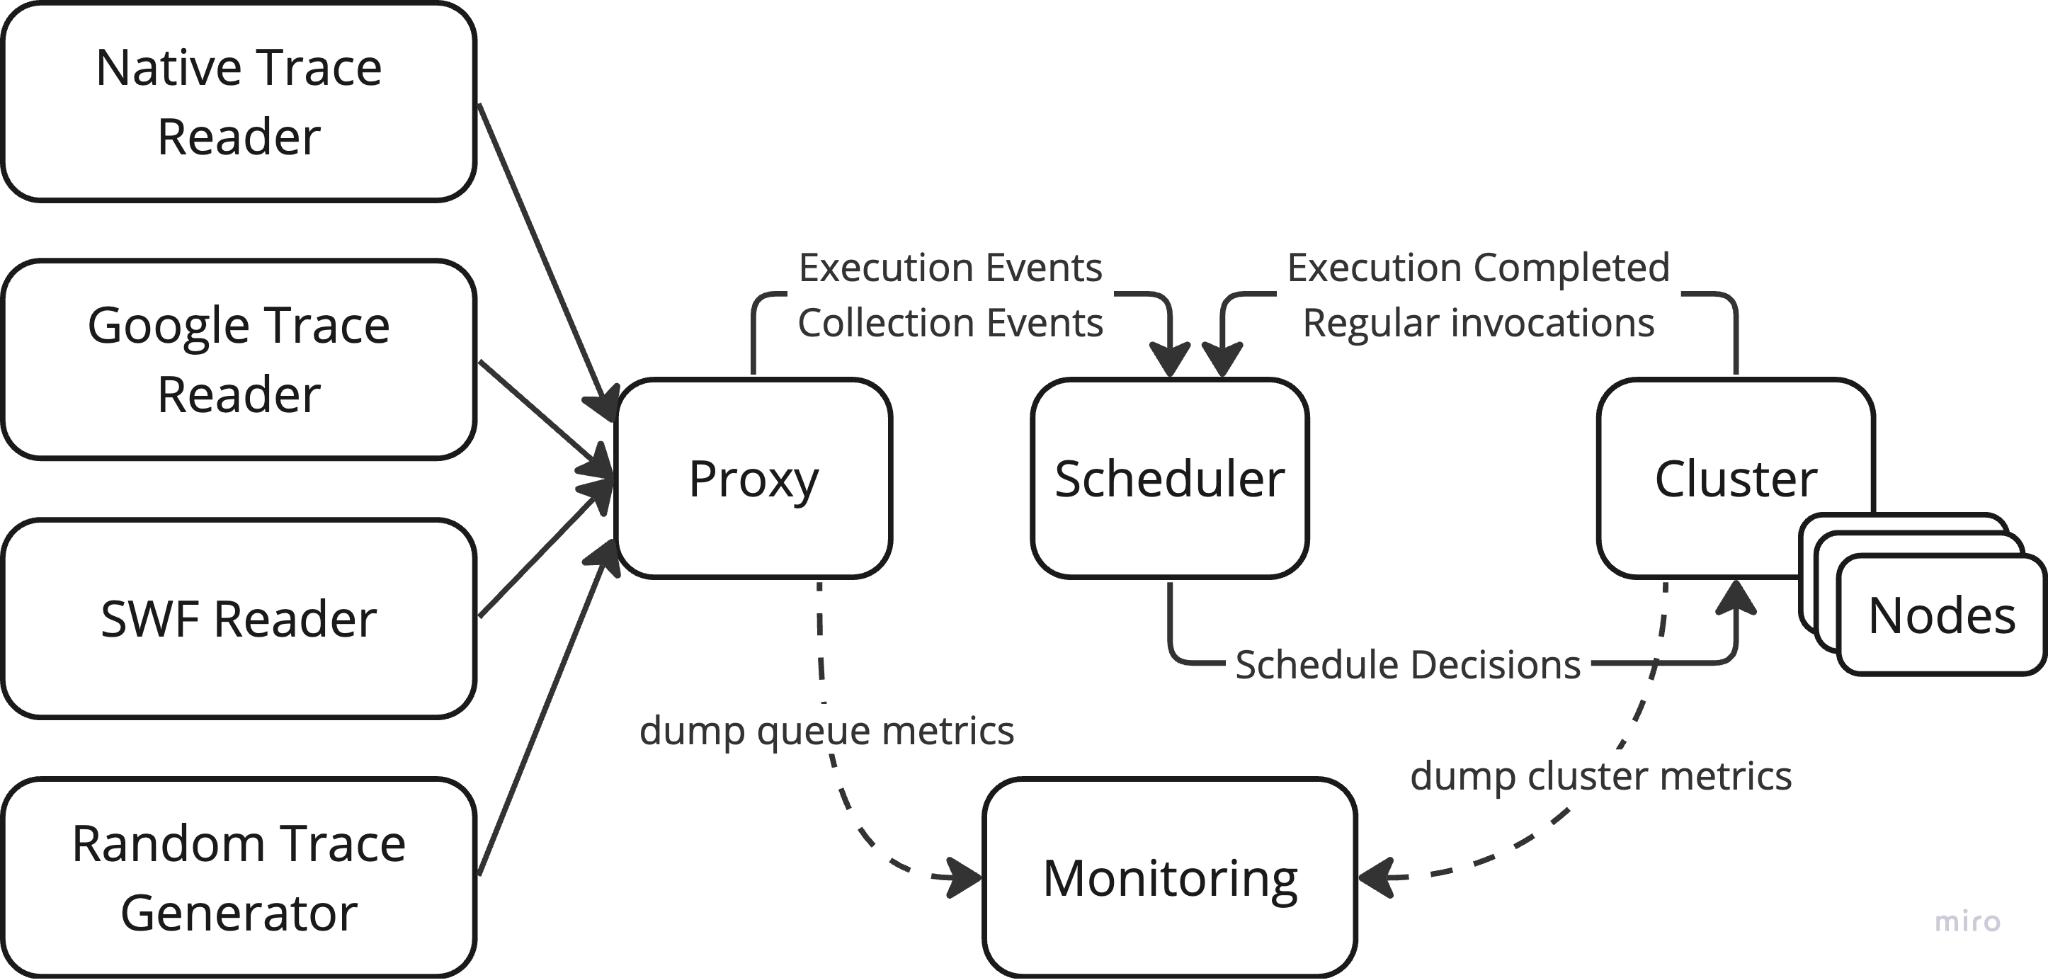
\includegraphics[width=0.8\textwidth]{images/simulator_arc}
    \caption{Архитектура симулятора}
    \label{fig:arch}
\end{figure}

Симулятор может работать в нескольких режимах, принимая на вход несколько видов входных данных. Это может быть как готовый трейс нагрузки из открытых источников (например, Google Trace), так и пользовательский ввод задач, описанный в виде JSON-файла.

Собирая информацию с компонентов \texttt{Proxy} и \texttt{Cluster} можно получить статистику о работе кластера и алгоритмов планирования. Например, насколько загружен кластер, насколько хорошо утилизируются его ресурсы. Такие выходные данные могут быть использованы для анализа работы алгоритмов и сравнения их эффективности. За это отвечает отдельный компонент -- \texttt{Monitoring}.


\subsection{Модель кластера}\label{cluster-model}
Вычислительный кластер -- это набор отдельных серверов, которые могут быть связаны между собой моделируемой сетью. 
В симуляторе используются готовые модули DSLab, из которых собирается каждый сервер (см. таблицу \ref{tab:server_modules}). 
\begin{table}[h]
    \centering
    \begin{tabular}{|l|l|c|}
    \hline
    \textbf{Название модуля} & \textbf{Используемый модуль} & \textbf{Обязательный} \\
    \hline
    \texttt{compute} & \texttt{dslab\_compute::multicore::Compute} & да \\
    \hline
    \texttt{network} & \texttt{dslab\_network::Network} & нет  \\
    \hline
    \texttt{disk} & \texttt{dslab\_storage::disk::Disk} & нет \\
    \hline
    \end{tabular}
    \caption{Модули каждого сервера в кластере}
    \label{tab:server_modules}
\end{table}


Подробнее с описанием этих модулей и примерами использования можно ознакомиться в официальной документации DSLab\cite{dslab-compute-docs}\cite{dslab-network-docs}\cite{dslab-storage-docs}.

\subsection{Вычислительная модель}\label{compute-model}

\subsubsection{Деление на Collection и Execution}

Поскольку симулятор может поддерживать несколько разных вычислительных моделей, для описания нагрузки был выбран обобщенный вариант: пользователь описывает задачи (\texttt{Execution}), которые непосредственно запускаются на кластере и потребляют ресурсы, и эти задачи могут быть связаны между собой заданием или коллекцией (\texttt{Collection}). Термин \texttt{Collection} происходит из аналогичного определения задания в последней версии Google Trace\cite{google-clusterdata}, а \texttt{Execution} является минимальной единицей планирования и может из себя представлять как простые вычисления, так и сложную программу, которой для запуска нужно одновременно выделить несколько серверов. Структуры данных представленны в таблицах \ref{tab:execution} и \ref{tab:collection}.

\begin{table}[h]
    \centering
    \label{tab:execution_request_fields}
    \begin{tabular}{|l|l|p{8cm}|}
        \hline
        \textbf{Поле} & \textbf{Тип} & \textbf{Описание} \\
        \hline
        id & \texttt{u64} & Уникальный идентификатор задачи на всю симуляцию \\
        \hline
        collection\_id & \texttt{Option<u64>} & Индекс задания или коллекции задач  \\
        \hline
        execution\_index & \texttt{Option<u64>} & Индекс задачи внутри задания/коллекции \\
        \hline
        time & \texttt{f64} & Время, когда задача становится доступной для планирования \\
        \hline
        schedule\_after & \texttt{Option<f64>} & Время, когда задача становится доступной для исполнения на кластере. Поле введено для поддержки совместимости с трейсом нагрузки из Google. \\
        \hline
        resources & \texttt{ResourceRequirements} & Структура требуемых ресурсов для исполнения задачи \\
        \hline
        profile & \texttt{Rc<dyn ExecutionProfile>} & Профиль нагрузки (см секцию \ref{sec:execution-profile}) \\
        \hline
        wall\_time\_limit & \texttt{Option<f64>} & Максимальное время на выполнение задачи, после которой она автоматически будет отменена \\
        \hline
        priority & \texttt{Option<u64>} & Приоритет задачи \\
        \hline
    \end{tabular}
    \caption{Описание \texttt{ExecutionRequest}}
    \label{tab:execution}
\end{table}

\begin{table}[h!]
    \centering
    \begin{tabular}{|l|l|p{8cm}|}
        \hline
        \textbf{Поле} & \textbf{Тип} & \textbf{Описание} \\ 
        \hline
        id & \texttt{u64} & Уникальный идентификатор задания/коллекции на всю симуляцию. \\
        \hline
        time & \texttt{f64} & Время, когда задание/коллекция становится известной планировщику. \\
        \hline
        user & \texttt{Option<String>} & Пользователь, который запускает эту коллекцию/задание. Используется для тестирования алгоритмов честного разделения кластера. \\
        \hline
        priority & \texttt{Option<u64>} & Приоритет приоритет задания/коллекции. Если у задачи указан собственный приоритет, то предполагается, что он переопределяет данный приоритет. \\
        \hline
    \end{tabular}
    \caption{Описание \texttt{CollectionRequest}}
    \label{tab:collection}
\end{table}

Описание требуемых ресурсов задачи состоит из требования к количеству хостов, а так же опционально к количеству ядер процессора и памяти на хостах. Таким образом, сохраняется возможность поддержать модель планирования аналогичной \texttt{BatSim}, \texttt{IRMaSim} и \texttt{Elastisim}, но и не упускается возможность для моделирования упаковки задач на кластерах (при указывании количества хостов больше одного,  есть возможность указать требования к ресурсам каждого хоста отдельно или всем сразу).

\subsubsection{ExecutionProfile}\label{sec:execution-profile}

Задачи, которые непосредственно выполняются на кластере, представляются в виде объектов, для которых реализован интерфейс \texttt{ExecutionProfile}:

\begin{figure}[h!]
    \small
\begin{rustcode}
pub trait ExecutionProfile {
  async fn run(self: Rc<Self>, processes: &Vec<HostProcessInstance>);
}
\end{rustcode}
\caption{Интерфейс \texttt{ExecutionProfile}}
\end{figure}

Метод \texttt{run} может быть реализован самим пользователем, но так же могут использоваться заготовки для простых сценариев работы. Такая задача получает в свое <<владение>> от планировщика набор выделенных аллокаций на узлах кластера и выполняет некоторую работу. Сама работа описывается в терминах асинхронного программирования на Rust и использует предоставленный интерфейс взаимодействия с кластером: 


\begin{figure}[h!]
    \small
\begin{rustcode}
    async fn sleep(&self, time: f64);
    async fn run_flops(&self, flops: f64);
    async fn transfer_data(&self, size: f64, dst_process: ProcessId);
    async fn write_data(&self, size: u64);
    async fn read_data(&self, size: u64);
\end{rustcode}
\caption{Интерфейс взаимодействия задачи с кластером}
\end{figure}

\subsection{Модель планирования заданий}

\subsection{Входные данные симуляции}

\subsection{Выходные данные симуляции}

\subsection{Конфигурация симуляции}

Вся настройка параметров симуляции происходит через конфигурационный файл в формате YAML. Пример конфигурации представлен на рисунке \ref{example-sim-config}. 

\begin{figure}[h!]
    \begin{yamlcode}
workload:
  - type: Native
    path: /path/to/trace
    options: 
      profiles_path: /path/to/profiles

hosts: 
  - count: 5
    cpus: 20
    memory: 20
    name_prefix: c
  - count: 5
    cpus: 5
    memory: 60
    name_prefix: m

monitoring:
  host_load_compression_time_interval: 100
  scheduler_queue_compression_time_interval: 100
  display_host_load: false 
  collect_user_queues: true

scheduler:
  hosts_invoke_interval: 10
\end{yamlcode}
\caption{Пример конфигурации симуляции}
\label{example-sim-config}
\end{figure}


\section{Эксперименты и тестирование}

\subsection{Производительность}

\subsection{Честность}

\section{Заключение}
